\documentclass[project.tex]{subfiles}
\begin{document}
\asubsection{5}{Проект интерфейса}
\par
Цвета:
\par
Цветовая схема интерфейса изменяется пользователем. На выбор представлены как светлые, так и темные варианты оформления.
\par
Шрифт:
\par
Для всего интерфейса выбран шрифт Jost. Это популярный шрифт без засечек, часто использующийся при разработке web-интерфейсов. В интерфейсе использованы начертания Bold (для заголовков), Regular и Light (для второстепенной информации).
\par
На каждой странице находится меню с ссылками на ключевые разделы и переключателем цветовой схемы интерфейса. На смартфонах навигацонное меню находится в верхней части экрана в виде «бургер-меню» (с возможностью сворачивания).
На устройствах с большей диагональю экрана меню представлено в виде боковой панели в левой части страницы.
\par
\vspace{0.5cm}
Интерфейс состоит из 10 страниц:
\begin{enumerate}
    \item «Список книг»\\
    Страница включает в себя список книг, представленных в виде карточек, включающих в себя обложку и основную информацию об издании, с указанием наличия электронной версии.
    Список разделен на страницы, переключение которых осуществляется при помощи кнопок, расположенных в нижней части страницы.
    В верхней части страницы находится строка поиска, панель фильтрации, кнопка «Случайная книга».
    \begin{figure}[H]
        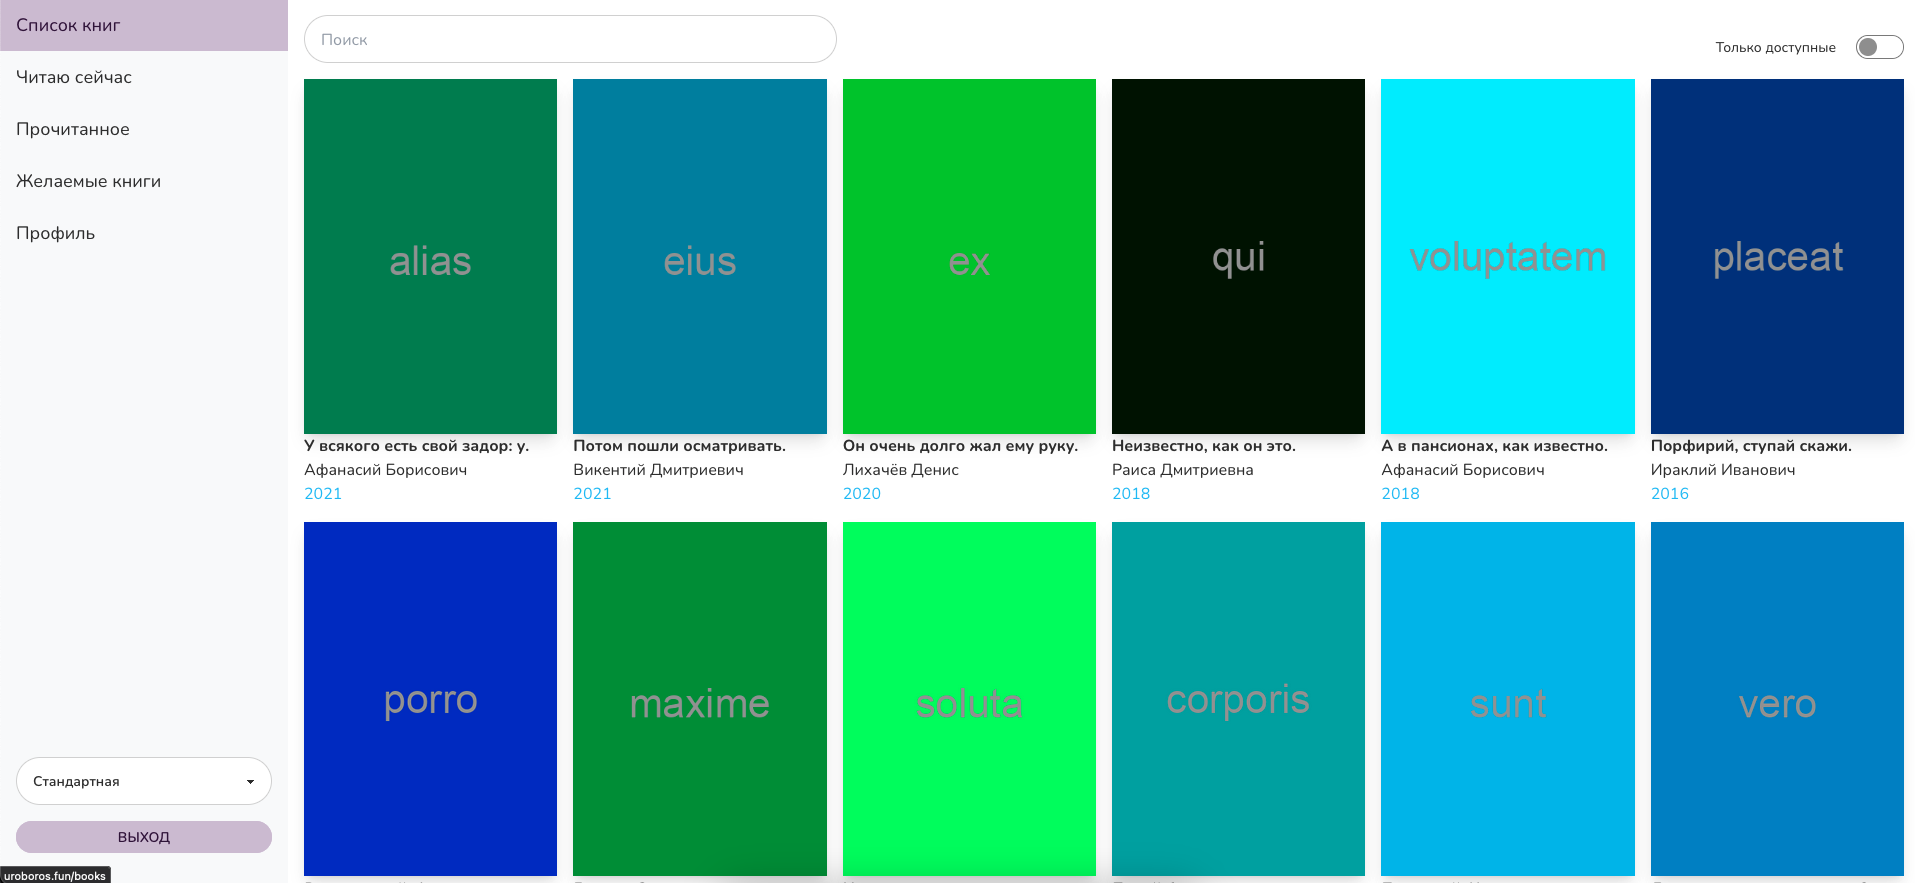
\includegraphics[width=\textwidth, frame]{../../graphics/mainpage.png}
        \caption{Страница "Список книг"}
        \label{pic:main}
    \end{figure}
    \item «Читаю сейчас»\\
    Страница включает в себя список книг, находящихся в текущий момент у Пользователя. Изданиям с истекшим сроком бронирования добавляется метка «Срок истек». Список книг выглядит как на рис. \ref{pic:main}.
    \item «Прочитанное»\\
    Страница включает в себя список книг, прочитанных Пользователем. При большом количестве элементов списка он разбивается на страницы, в нижней части появляются кнопки для переключения текущей страницы. Список книг выглядит как на рис. \ref{pic:main}.
    \item Страница книги\\
    На странице книги отображена более детальная информация: обложка, название, автор, описание, теги, год публикации и количество страниц.
    \par
    Пользователь может просмотреть историю бронирований и возвратов каждого из экземпляров книги, с указанием даты бронирования/возврата и ФИО Пользователей.
    \par
    Если для книги загружено электронное издание, появляется ссылка на его скачивание.
    \par
    Если выбранный экземпляр доступен для взятия, появляется кнопка «Взять», при нажатии на которую добавится запись в читательскую карточку и историю бронирований.
    \par
    Если экземпляр книги в текущий момент закреплен за Пользователем, появляется кнопка «Вернуть», при нажатии на которую добавится соответствющая запись в читательскую карточку и историю бронирований. Книга станет доступной для бронирования.
    \par
    Если экземпляр книги в текущий момент закреплен за другим Пользователем, появляется кнопка «В лист ожидания», при нажатии на которую Пользователь добавляется в очередь на взятие книги.
    \par
    Если страницу просматривает Администратор, ему доступны кнопки редактирования и удаления книги, добавления и удаления экземпляров.
    \par
    В нижней части страницы размещен раздел «Отзывы». Он состоит из формы для добавления отзыва и списка отзывов. Пользователь может удалить собственный отзыв, Администратор может удалять все отзывы.
    \begin{figure}[H]
       \label{pic:book}
       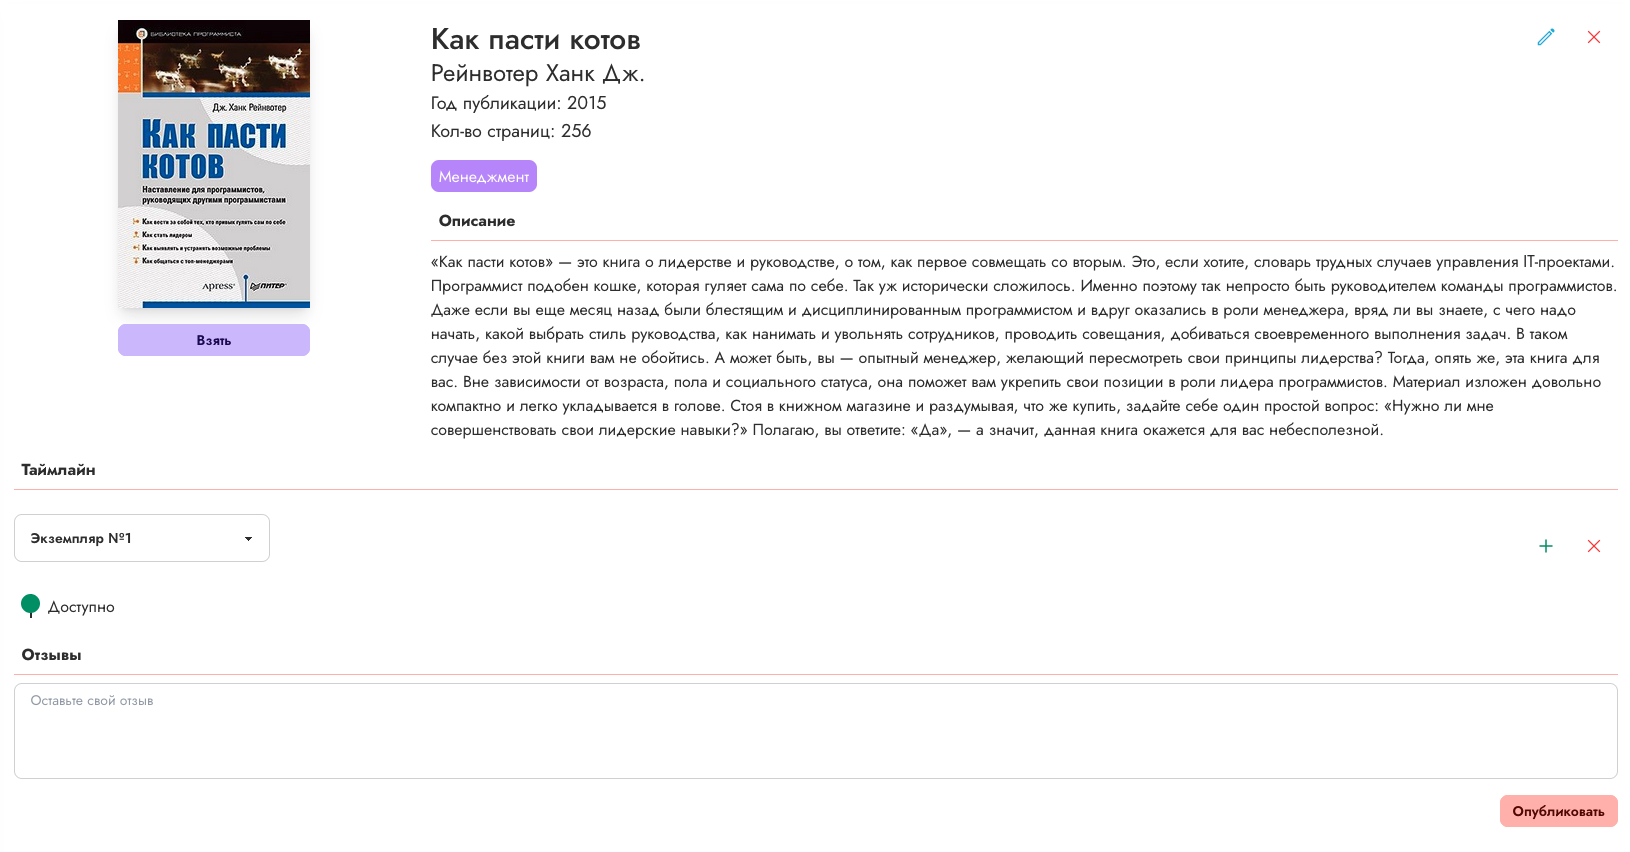
\includegraphics[width=\textwidth, frame]{../../graphics/singlebook.png}
       \caption{Страница книги} 
    \end{figure}
    \begin{figure}[H]
       \label{pic:states}
       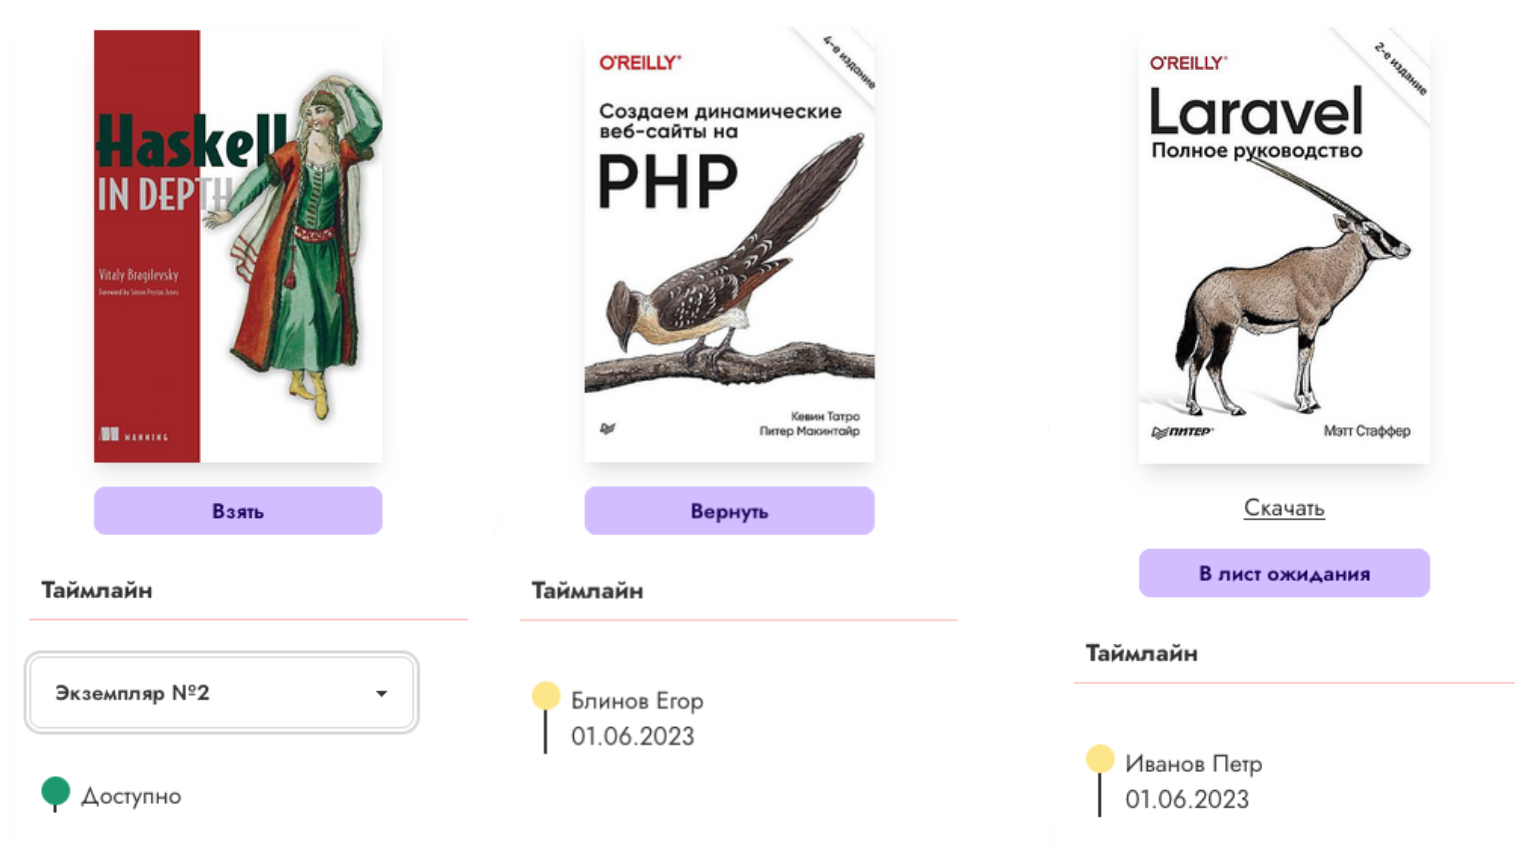
\includegraphics[width=\textwidth, frame]{../../graphics/bookstates.png}
       \caption{Состояния книги: доступна, читаю сейчас, занята} 
    \end{figure}
    \item «Желаемые книги»\\
    На странице находятся книги, которые Пользователи хотели бы видеть в библиотеке. В верхней части экрана расположена поисковая строка и кнопка «Добавить книгу». Также все Пользователи могут голосовать за понравившиеся книги, используя кнопку, находяющуюся на карточке издания. Так, ответственный за их закупку сможет отследить интересы и потребности коллег. 
    При большом количестве элементов списка он разбивается на страницы, в нижней части появляются кнопки для переключения текущей страницы.
    \begin{figure}[H]
       \label{pic:desired}
       \centering{
       
\includegraphics[width=0.5\textwidth, frame]{../../graphics/desired_list.png}
       }
       \caption{Желаемые книги} 
    \end{figure}
    \item Страница добавления книги\\
    Доступна только для Администратора. Страница состоит из формы, включающей набор полей ввода информации о книге. На мобильных устройствах доступен сканер ISBN, для автоматизированного получения информации о книге с помощью Google Books API. При сохранении книга добавится в основной список книг.
    \begin{figure}[H]
       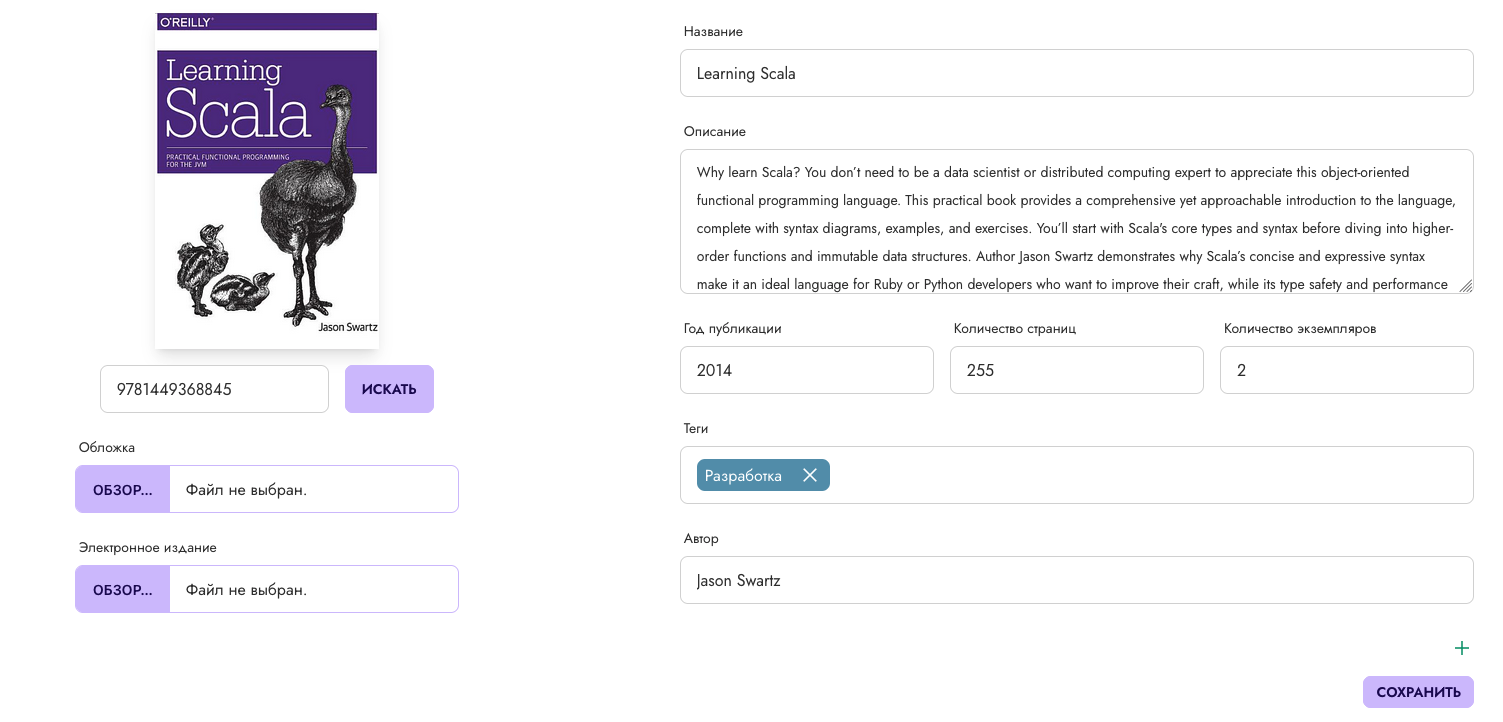
\includegraphics[width=\textwidth, frame]{../../graphics/bookform.png}
       \caption{Страница добавления книги} 
       \label{pic:form}
    \end{figure}
    \item Страница добавления книги в раздел «Желаемые книги»\\
    Страница состоит из формы, включающей набор полей ввода информации о книге. После сохранения книга будет отображаться в разделе «Желаемые книги». Интерфейс представлен на рис. \ref{pic:form}.
    \item Страница книги из раздела «Желаемые книги»\\
    На странице книги отображена более детальная информация о запрашиваемой книге: обложка, название, автор, описание, год публикации и количество страниц. Также отображается ФИО человека, добавившего книгу. Администратору доступна кнопка «В список книг», которую следует нажимать после приобретения издания. Так, книга перестанет отображаться в разделе «Желаемые книги» и станет доступна для бронирования Пользователями в общем списке книг.
    \item «Настройки»\\
    Страница доступна только для Администратора. Доступны поля ввода для редактирования максимального срока бронирования и установления лимита бронирований книг Пользователями, интерфейс для редактирования списка тегов.
    \par
    Также Администратор может просмотреть список всех текущих бронирований, список «должников».
    \begin{figure}[H]
       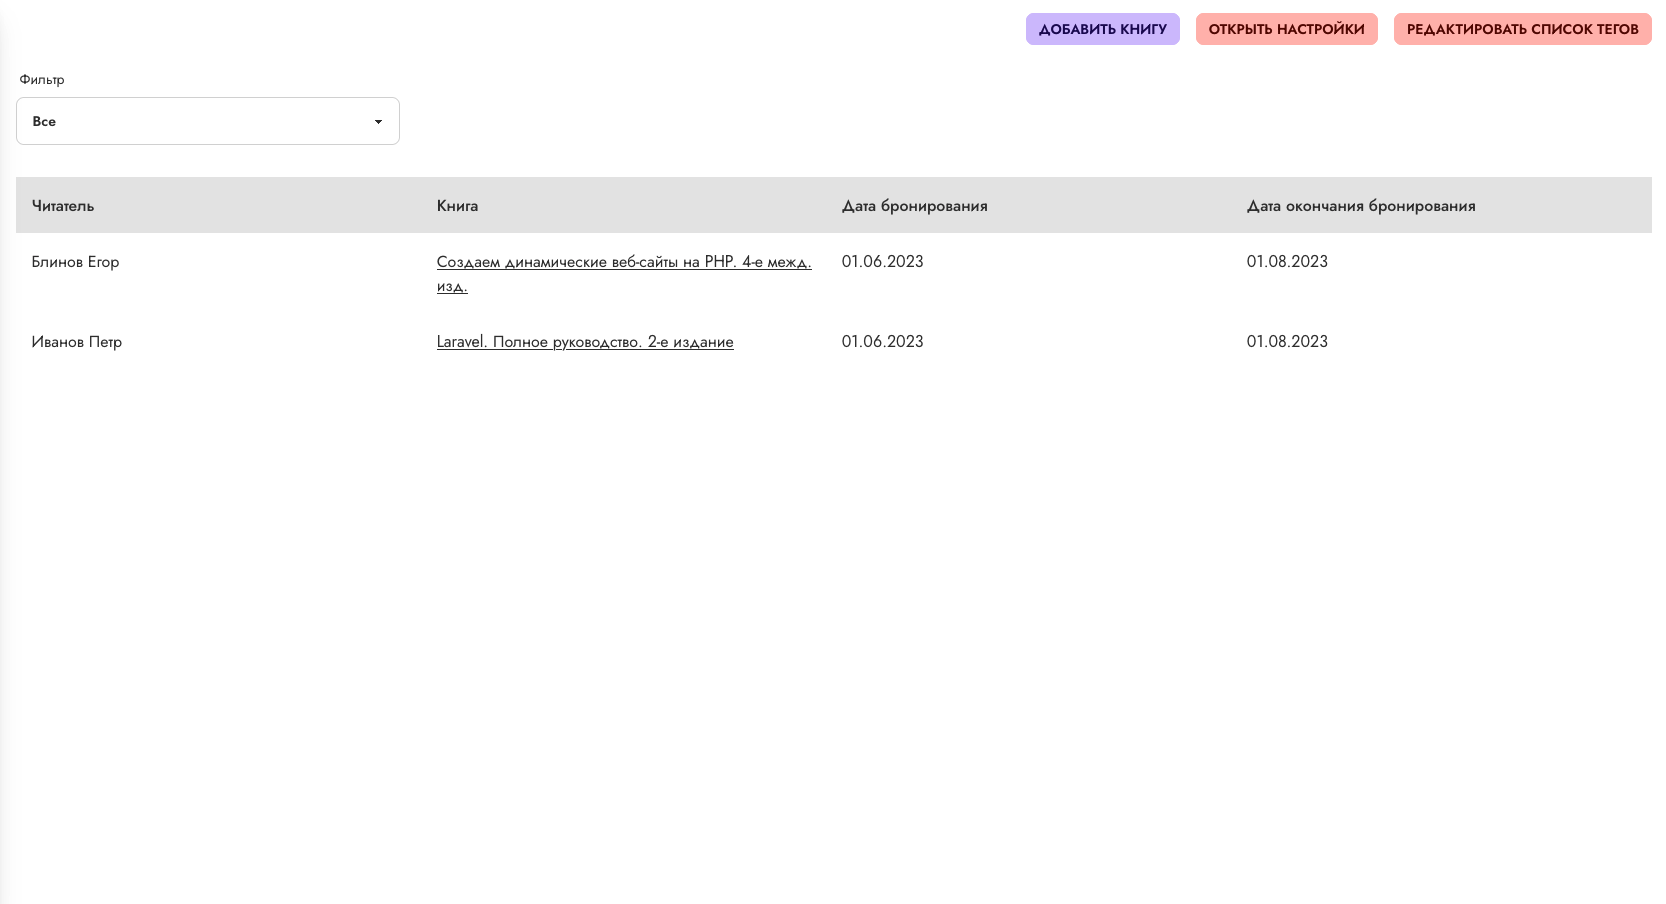
\includegraphics[width=\textwidth, frame]{../../graphics/settings.png}
       \caption{Страница «Настройки»} 
       \label{pic:settings}
    \end{figure}
    \item «Профиль»\\
    На странице доступны чекбоксы для получения уведомлений об истечении срока бронирований и новых книгах.
\end{enumerate}
\end{document}